\documentclass[12pt,a4paper]{article}
\usepackage{amsmath,amssymb,graphicx,cite}
\usepackage{cite}
\bibliographystyle{iopart-num}

\begin{document}

\section{Focusing of vector beams}
The properties of highly focused polarised beams can be numerically analysed with the Richards-Wolf vectorial diffraction method \cite{richards_wolf}. Here we consider the focusing of spatially inhomogeneous (vector) beams of axial symmetry; the derivation of the electric field at or near the focus most closely follows that of Youngworth \& Brown \cite{youngworth_brown}, and Zhan \cite{zhan}. The geometry of our problem is shown in Fig.~\ref{fig:setup}. The incident electric field may have any spatially prescribed amplitude and polarisation distribution, and we assume a planar phase front over the entrance pupil.
\begin{figure}[h]
	\centering
	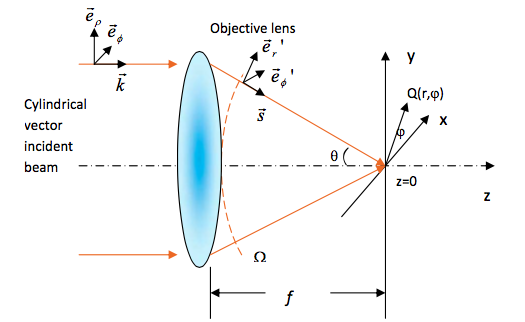
\includegraphics[width=12cm]{setup} 
	\caption{Focusing of a cylindrical vector beam. \(Q\!\left(r,\varphi,z\right)\) is an observation point in the focal plane.}
	\label{fig:setup}
\end{figure}

The incident field can be written in pupil plane cylindrical coordinates \(\left(\rho,\phi,z\right)\) as
\begin{displaymath}
	\mathbf{E}^{(i)}\!\left(\rho,\phi\right) = l_{0}P\!\left(\rho\right)\left[E_{\rho}^{(i)}\mathbf{e}_{\rho} + E_{\phi}^{(i)}\mathbf{e}_{\phi}\right]
\end{displaymath}
where \(l_{0}\) is the peak field amplitude and \(P\!\left(\rho\right)\) is the axially symmetric pupil plane amplitude distribution normalised to \(l_{0}\). The unit vectors \(\mathbf{e}_{\rho}\) and \(\mathbf{e}_{\phi}\) can be expressed in Cartesian coordinates as
\begin{align}
		\mathbf{e}_{\rho} &= \cos{\phi}\:\mathbf{e}_{x} + \sin{\phi}\:\mathbf{e}_{y}, \nonumber \\
		\mathbf{e}_{\phi} &= \mathbf{e}_{\rho}\times\hat{\mathbf{k}} = \sin{\phi}\:\mathbf{e}_{x} - \cos{\phi}\:\mathbf{e}_{y}. \nonumber
\end{align}
An aplanatic lens produces a spherical wave converging at the focal point. We assume the lens obeys the sine condition and thus the amplitude distribution over the pupil is mapped onto the spherical wavefront through \(\rho=f\sin{\theta}\) where \(f\) is the focal length of the lens. Power conservation requires (consider changing basis from a cylindrical \(\left(\rho,\phi\right)\) to a spherical \(\left(r,\phi,\theta\right)\) coordinate system) 
\begin{displaymath}
	P^{2}\!\left(\rho\right)2\pi\rho d\rho = P^{2}\!\left(\theta\right)2\pi f^{2}\sin{\theta}d\theta .
\end{displaymath}
From here, it is easily verified that
\begin{displaymath}
	P\!\left(\theta\right) = P\!\left(f\sin{\theta}\right)\sqrt{\cos{\theta}} .
\end{displaymath}
The function \(P\!\left(\theta\right)\) is termed the `apodization function' and encodes information about the transverse amplitude distribution of the incoming beam (see later).

Following Richards and Wolf, we may express the electric field near the focus as a diffraction integral over the vector field amplitude \(\mathbf{a}\!\left(\theta,\phi\right)\) on the spherical wavefront with focal radius \(f\):
\begin{equation}
	\label{eq:rw}
	\mathbf{E}\!\left(r,\phi,z\right) = \frac{-ik}{2\pi} \iint_\Omega \mathbf{a}\!\left(\theta,\phi\right) e^{ik\left(\mathbf{s}\cdot\mathbf{r}\right)}d\Omega
\end{equation}
where the field strength factor \(\mathbf{a}\) is given by
\begin{equation}
	\label{eq:strfct}
	\mathbf{a}\!\left(\theta,\phi\right) = l_{0}fP\!\left(\theta\right)\left[E_{\rho}^{(i)}\mathbf{e}_{r}^{\prime} + E_{\phi}^{(i)}\mathbf{e}_{\phi}^{\prime}\right]
\end{equation}
where \(k\) is the wavenumber and \(\mathbf{r}=\!\left(r,\varphi,z\right)\) denotes a point in the image space. After refraction, the new basis vectors are found through geometrical considerations as
\begin{align}
	\mathbf{e}_{r}^{\prime} &= \cos{\theta}\left(\cos{\phi}\:\mathbf{e}_{x} +\sin{\phi}\:\mathbf{e}_{y}\right) + \sin{\theta}\:\mathbf{e}_{z}, \\
	\hat{\mathbf{s}} &= \sin{\theta}\left(\cos{\phi}\:\mathbf{e}_{x} + \sin{\phi}\:\mathbf{e}_{y}\right) + \cos{\theta}\:\mathbf{e}_{z}, \\
	\label{eq:azi}
	\mathbf{e}_{\phi}^{\prime} &= \mathbf{e}_{r}^{\prime} \times \hat{\mathbf{s}} = \sin{\phi}\cos{2\theta}\:\mathbf{e}_{x} - \cos{\phi}\cos{2\theta}\:\mathbf{e}_{y},
\end{align}
and we have
\begin{equation}
	\label{eq:exponent}
	\mathbf{s}\cdot\mathbf{r} = z\cos{\theta}+r\sin{\theta}\cos{\left(\varphi - \phi\right)}.
\end{equation}
We note here that Eq.~\eqref{eq:azi} differs from both Zhan and Youngworth \& Brown who erroneously took \(\textbf{e}_{\phi}^{\prime} = \textbf{e}_{\phi}\) (i.e. did not perform the cross product) and thus miss the \(\cos{\left(2\theta\right)}\) term.

Now substituting Eqs.~\eqref{eq:strfct}--\eqref{eq:exponent} into Eq.~\eqref{eq:rw} we find
\begin{multline}
	\label{eq:rwsub}
	\mathbf{E}\!\left(r,\varphi,z\right) = \frac{-ik}{2\pi} \int_{0}^{\alpha}\int_{0}^{2\pi}l_{0}fP\!\left(\theta\right)\cos^{\frac{1}{2}}\!{\theta}\sin{\theta}e^{ik\left(z						\cos{\theta}+r\sin{\theta}\cos{\left(\varphi - \phi\right)}\right)}\\
	\Bigg[E_{\rho}^{(i)}\begin{pmatrix}\cos{\theta}\cos{\phi}\:\textbf{e}_{x}\\ \cos{\theta}\sin{\phi}\:\textbf{e}_{y}\\ \sin{\theta}\:\textbf{e}_{z} \end{pmatrix}+E_{\phi}^{(i)}\begin{pmatrix}\cos{2\theta}\sin{\phi}\:\textbf{e}_{x}\\ -	\cos{2\theta}\cos{\phi}\:\textbf{e}_{y} \\ 0\:\textbf{e}_{z} \end{pmatrix}\Bigg] d\theta d\phi,
\end{multline}
where we have explicitly included the integrals over the polar and azimuthal angles, and introduced \(\alpha\) as the angular extent of the aperture. We now change from Cartesian coordinates into image plane cylindrical coordinates through
\begin{align}
		\mathbf{e}_{r} &= \cos{\varphi}\:\mathbf{e}_{x} + \sin{\varphi}\:\mathbf{e}_{y}, \nonumber \\
		\mathbf{e}_{\varphi} &= \sin{\varphi}\:\mathbf{e}_{x} - \cos{\varphi}\:\mathbf{e}_{y}, \nonumber
\end{align}
giving
\begin{multline}
	\label{eq:final}
	\mathbf{E}\!\left(r,\varphi,z\right) = \frac{-iA}{\pi} \int_{0}^{\alpha}\int_{0}^{2\pi}P\!\left(\theta\right)\cos^{\frac{1}{2}}\!{\theta}\sin{\theta}e^{ik\left(z						\cos{\theta}+r\sin{\theta}\cos{\left(\varphi - \phi\right)}\right)}\\
	\Bigg[E_{\rho}^{(i)}\begin{pmatrix}\cos{\theta}\cos{\left(\phi-\varphi\right)}\:\textbf{e}_{r}\\ 0\:\textbf{e}_{\varphi}\\ \sin{\theta}\:\textbf{e}_{z} \end{pmatrix}+E_{\phi}^{(i)}\begin{pmatrix} 0\:\textbf{e}_{r}\\ \cos{2\theta}\cos{\left(\phi-\varphi\right)}\:\textbf{e}_{\varphi} \\ 0\:\textbf{e}_{z} \end{pmatrix}\Bigg] d\theta d\phi,
\end{multline}
where
\begin{displaymath}
	A = \frac{\pi f l_{0}}{\lambda}.
\end{displaymath}
Note that the radial component of the incident beam contributes to the radial and longitudinal field components near the focal plane, while the azimuthal component in the incident beam contributes only to the azimuthal field component near the focal plane.

We can further simplify the expression using the identity
\begin{displaymath}
	\int_{0}^{2\pi}\cos{\left(n\psi\right)}e^{ikr\sin{\theta}\cos{\psi}}d\phi = 2\pi i^{n}J_{n}\!\left(kr\sin{\theta}\right)
\end{displaymath}
where \(J_{n}\!\left(x\right)\) is the Bessel function of the first kind with order \(n\). Finally, selecting each component individually by appropriately choosing \(E_{\rho}^{(i)}\) and \(E_{\phi}^{(i)}\) as zero or one, we find:
\begin{align}
	\label{eq:er}
	E_{r}\!\left(r,\varphi,z\right) &= A\int_{0}^{\alpha} P\!\left(\theta\right)\cos^{\frac{1}{2}}\!{\theta}\sin{2\theta}J_{1}\!\left(kr\sin{\theta}\right)e^{ikz\cos{\theta}}d\theta, \\
	\label{eq:ephi}
	E_{\varphi}\!\left(r,\varphi,z\right) &= 2A\int_{0}^{\alpha} P\!\left(\theta\right)\cos^{\frac{1}{2}}\!{\theta}\sin{\theta}\cos{2\theta}J_{1}\!\left(kr\sin{\theta}\right)e^{ikz\cos{\theta}}d\theta, \\
	\label{eq:ez}
		E_{z}\!\left(r,\varphi,z\right) &= 2iA\int_{0}^{\alpha} P\!\left(\theta\right)\cos^{\frac{1}{2}}\!{\theta}\sin^{2}{\theta}J_{0}\!\left(kr\sin{\theta}\right)e^{ikz\cos{\theta}}d\theta.
\end{align}

We require now only to find the apodization function, \(P\!\left(\theta\right)\), which was alluded to earlier. The standard scalar Helmholtz equation, often used in the paraxial approximation, is inadequate for describing spatially inhomogeneous beam polarisations. Following the procedure of Jordan and Hall \cite{jordan_hall}, consider the full vector wave equation
\begin{displaymath}
	\nabla\times\nabla\times\mathbf{E} -k^{2}\mathbf{E} = 0.
\end{displaymath}
Assuming implicit time dependence, and an azimuthally symmetric solution of the form
\begin{displaymath}
	\mathbf{E}\!\left(\rho,z\right)=\hat{\boldsymbol{\varphi}}U\!\left(\rho,z\right)=\hat{\boldsymbol{\varphi}}f\!\left(\rho,z\right)e^{ikz},
\end{displaymath}
we can substitute to find the following scalar equation for the azimuthal beam component:
\begin{displaymath}
	\frac{\partial^{2}\!f}{\partial \rho^{2}}+	\frac{1}{\rho}\frac{\partial f}{\partial\rho}+\frac{\partial^{2}\!f}{\partial z^{2}}+2ik\frac{\partial f}{\partial z}-\frac{f}{\rho^{2}}=0.
\end{displaymath}
From here we make the paraxial approximation to give
\begin{equation}
	\label{eq:azisw}
	\frac{\partial^{2}\!f}{\partial \rho^{2}}+	\frac{1}{\rho}\frac{\partial f}{\partial \rho}+2ik\frac{\partial f}{\partial z}-\frac{f}{\rho^{2}}=0.
\end{equation}
Note the similarity between Eq.~\eqref{eq:azisw} and the usual paraxial scalar wave equation --- differing only by the \(-f/\rho^{2}\) term. Eq.~\eqref{eq:azisw} is also reminiscent of Bessel's equation of order one and indeed a solution is found at the plane \(z=0\) of
\begin{equation}
	\label{eq:aziswsol}
	f\!\left(\rho,0\right)\sim J_{1}\!\left(\beta \rho\right)e^{-(\rho/w_{0})^{2}},
\end{equation}
where \(w_{0}\) is the (input) beam waist and \(\beta=k\sin{\Theta}\) (\(\Theta\) is the angular half-aperture of the beam cone) is described by Gori et. al. \cite{gori} as `the length of the component, orthogonal to the z-axis, of any wave vector belonging to one of the plane waves producing the beam'. Eq.~\eqref{eq:aziswsol} gives the normalised electric field amplitude at the beam waist, i.e. in the beam \(z=0\) plane which we can take as the focal plane. Our system obeys the sine condition, so we have \(\rho=f\sin{\theta}\), and since Eq.~\eqref{eq:aziswsol} obeys azimuthal symmetry, it can be cast in a form appropriate for the integrals in Eqs.~\eqref{eq:er}--\eqref{eq:ez}:
\begin{displaymath}
	f\!\left(\rho,0\right)\to P\!\left(\theta\right)=J_{1}\!\left(\beta f\sin{\theta}\right)e^{-(f\sin{\theta}/w_{0})^{2}}.
\end{displaymath}
Finally, since the aperture radius of the lens is \(f\sin{\alpha}\), we can define the filling factor \(f_{0}\) as
\begin{displaymath}
	f_{0}= \frac{f\sin{\alpha}}{w_{0}}
\end{displaymath}
which gives
\begin{equation}
	\label{eq:apod}
	P\!\left(\theta\right)=J_{1}\!\left(\beta f\sin{\theta}\right)e^{-(f_{0}\sin{\theta}/\sin{\alpha})^{2}}.
\end{equation}
Eq.~\eqref{eq:apod} is the final form of the apodization function and can essentially be viewed as a pupil filter. We are now able to numerically evaluate Eqs.~\eqref{eq:er}--\eqref{eq:ez}. These components also form an orthogonal basis; for any arbitrary input field, we can decompose the polarisation at each point on the beam profile into a combination of \((r,\varphi,z)\) components which can be propagated through the system by Eqs.~\eqref{eq:er}--\eqref{eq:ez} and recombined at the focus. This allows us to simulate not only entirely radially or azimuthally polarised beams but also (interesting) linear combinations.
\section{Propagation}
The next natural question to ask is this: what does a given field at the focus look like in the far field? Specifically, how can we propagate this field beyond the range in which Eqs.~\eqref{eq:er}--\eqref{eq:ez} are valid (only a few wavelengths)? To begin answering this, we look to Goodman \cite{goodman} and Novotny \& Hecht \cite{hecht_nov}.

We formulate these ideas using scalar diffraction theory. From Goodman: ``\emph{if the complex field distribution of a monochromatic disturbance is Fourier-analysed across any plane, the various spatial Fourier components can be identified as plane waves travelling in different directions away from that plane. The field amplitude at any other point (or across any other parallel plane) can be calculated by adding the contribution of these plane waves, taking due account of the phase shifts undergone during propagation}".

Suppose that some wave is incident on a transverse \((x,y)\) plane travelling with a component of propagation in positive \(z\). Let the complex field across a plane \(z=0\) be \(U(x,y,0)\) where this scalar field could denote any polarisation; our goal is to find \(U(x,y,z)\). Across the \(z=0\) plane, \(U\) has a two-dimensional Fourier transform given by
\begin{displaymath}
	A\!\left(f_{x},f_{y};0\right)=\iint_{\infty}^{\infty}U\!\left(x,y,0\right)\exp\left[-2\pi i\left(f_{x}x+f_{y}y\right)\right]dxdy
\end{displaymath}
where \(f_{x},f_{y}\) are spatial frequencies. Equivalently, we can write \(U\) as an inverse Fourier transform:
\begin{equation}
	\label{eq:fourier}
	U\!\left(x,y,0\right)=\iint_{\infty}^{\infty}A\!\left(f_{x},f_{y};0\right)\exp\left[2\pi i\left(f_{x}x+f_{y}y\right)\right]df_{x}df_{y}.
\end{equation}
To shed physical insight on this, consider a simple plane wave propagating with wavevector \(\mathbf{k}\) that has magnitude \(2\pi/\lambda\) and directional cosines \(\left(\alpha,\beta,\gamma\right)\) such that 
\begin{displaymath}
	\alpha=\frac{k_{x}}{k}, \beta=\frac{k_{y}}{k}, \gamma=\frac{k_{z}}{k}
\end{displaymath}
and \(\alpha^{2}+\beta^{2}+\gamma^{2}=1\). Such a plane wave has complex representation of the form \(\exp\!\left[i\left(\mathbf{k}\cdot\mathbf{r}-\omega t\right)\right]\) where the position vector \(\mathbf{r}=x\mathbf{e}_{x}+y\mathbf{e}_{y}+z\mathbf{e}_{z}\) and 
\begin{displaymath}
	\mathbf{k}=\frac{2\pi}{\lambda}\left(\alpha \mathbf{e}_{x}+\beta \mathbf{e}_{y}+\gamma \mathbf{e}_{z}\right).
\end{displaymath}
Dropping the time dependence and evaluating explicitly, we have a spatial dependence of
\begin{displaymath}
	\exp\left[i\frac{2\pi}{\lambda}\left(\alpha x+\beta y+\gamma z\right)\right].
\end{displaymath}
Thus across a plane \(z=0\), a complex exponential function \(\exp\left[2\pi i\left(f_{x}x+f_{y}y\right)\right]\)	may be regarded as representing a plane wave propagating with directional cosines
\begin{displaymath}
	\alpha=\lambda f_{x},\:\beta=\lambda f_{y},\:\gamma=\sqrt{1-\left(\lambda f_{x}\right)^{2}-\left(\lambda f_{y}\right)^{2}}.
\end{displaymath}
Eq.~\eqref{eq:fourier}, the Fourier decomposition of \(U\), we can now be regarded as the summation of an infinite number of plane waves, evaluated at spatial frequencies \(f_{x}=\alpha/\lambda, f_{y}=\beta/\lambda\) and with complex amplitudes \(A\left(f_{x},f_{y};0\right)df_{x}df_{y}\). Hence the function
\begin{equation}
	\label{eq:angspec}
	A\!\left(\frac{\alpha}{\lambda},\frac{\beta}{\lambda};0\right)=\iint_{\infty}^{\infty}U\!\left(x,y,0\right)\exp\left[-2\pi i\left(\frac{\alpha}{\lambda}x+\frac{\beta}{\lambda}y\right)\right]dxdy
\end{equation}
is called the \emph{angular spectrum} of \(U(x,y,0)\).

Consider now the angular spectrum of a disturbance \(U(x,y,z)\), denoted \(A\left(\frac{\alpha}{\lambda},\frac{\beta}{\lambda};z\right)\):
\begin{displaymath}
	A\!\left(\frac{\alpha}{\lambda},\frac{\beta}{\lambda};z\right)=\iint_{\infty}^{\infty}U\!\left(x,y,z\right)\exp\left[-2\pi i\left(\frac{\alpha}{\lambda}x+\frac{\beta}{\lambda}y\right)\right]dxdy
\end{displaymath}
We wish to find the relation between \(A\left(\frac{\alpha}{\lambda},\frac{\beta}{\lambda};0\right)\) and \(A\left(\frac{\alpha}{\lambda},\frac{\beta}{\lambda};z\right)\). Note we can write
\begin{equation}
	\label{eq:angspec1}
	U\!\left(x,y,z\right)=\iint_{\infty}^{\infty}A\!\left(\frac{\alpha}{\lambda},\frac{\beta}{\lambda};z\right)\exp\left[2\pi i\left(\frac{\alpha}{\lambda}x+\frac{\beta}{\lambda}y\right)\right]d\frac{\alpha}{\lambda}d\frac{\beta}{\lambda}
\end{equation}
which must satisfy the scalar Helmholtz equation
\begin{equation}
	\label{eq:scalhelm}
	\nabla^{2}U+k^{2}U=0
\end{equation}
at all source free points. Direct substitution of Eq.~\eqref{eq:angspec1} into Eq.~\eqref{eq:scalhelm} gives the following requirement:
\begin{displaymath}
	\frac{d^{2}}{dz^{2}}A\!\left(\frac{\alpha}{\lambda},\frac{\beta}{\lambda};z\right)+\left(\frac{2\pi}{\lambda}\right)^{2}\left(1-\alpha^{2}-\beta^{2}\right)A\!\left(\frac{\alpha}{\lambda},\frac{\beta}{\lambda};z\right)=0,
\end{displaymath}
to which we immediately find an elementary solution of
\begin{equation}
	\label{propasol}
	A\!\left(\frac{\alpha}{\lambda},\frac{\beta}{\lambda};z\right)=A\!\left(\frac{\alpha}{\lambda},\frac{\beta}{\lambda};0\right)\exp\left[\pm i\frac{2\pi}{\lambda}z\sqrt{1-\alpha^{2}-\beta^{2}}\right].
\end{equation}
This result demonstrates that when direction cosines \(\alpha,\beta\) satisfy \(\alpha^{2}+\beta^{2}<1\) (i.e. non-evanescent), the effect of propagation is simply a change in the relative phase of each of component in the angular spectrum. Note the positive and negative exponent solutions in Eq.~\eqref{propasol} refer to propagation in the positive and negative \(z\) directions, respectively. Since each plane-wave component propagates at a different angle, each travels a different distance between parallel planes, and relative phase delays are introduced.

We can now inverse transform to deduce the disturbance at \((x,y,z)\):
\begin{multline}
	\label{propa}
	U\!\left(x,y,z\right)=\iint_{\infty}^{\infty}A\!\left(\frac{\alpha}{\lambda},\frac{\beta}{\lambda};0\right)\exp\left[\pm i\frac{2\pi}{\lambda}z\sqrt{1-\alpha^{2}-\beta^{2}}\right]	\\				\exp\left[2\pi i\left(\frac{\alpha}{\lambda}x+\frac{\beta}{\lambda}y\right)\right]d\frac{\alpha}{\lambda}d\frac{\beta}{\lambda}.
\end{multline}
Finally, we can write this in the more intuitive wavenumber space by recognising \(\alpha/\lambda=k_{x}/2\pi\) and so on, giving:
\begin{equation}
	\label{propafinal}
	U\!\left(x,y,z\right)=\frac{1}{4\pi^{2}}\iint_{\infty}^{\infty}A\!\left(k_{x},k_{y};0\right)	\exp\left[i\left(k_{x}x+k_{y}y\pm k_{z}z\right)\right]dk_{x}dk_{y}
\end{equation}
where
\begin{equation}
	\label{fourierfinal}
	A\!\left(k_{x},k_{y};0\right)=\iint_{\infty}^{\infty}U\!\left(x,y,0\right)\exp\left[-i\left(k_{x}x+k_{y}y\right)\right]dxdy.
\end{equation}
This allows us to take any complex field and propagate it to any distance. However by using only scalar diffraction theory, we have not taken the full vectorial nature of light into account, and thus Eq.~\eqref{propafinal} may not be suitable for fields with for example a very large longitudinal component. Further study is require here.

\bibliography{dl_vbeams}

\end{document}